\documentclass[a4paper,14pt]{extarticle}

\usepackage[left=30mm, right=10mm, top=20mm, bottom=20mm]{geometry}

\usepackage[T2A]{fontenc}
\usepackage[utf8]{inputenc}
\usepackage[russian]{babel}
\usepackage{tempora}
\usepackage{type1cm}
\usepackage{indentfirst}

\usepackage{minted}
\usepackage{xcolor}

\usepackage{siunitx}
\usepackage{booktabs}
\usepackage{multirow}


\usepackage{csquotes}
\usepackage[
    parentracker=true,
    backend=biber,
    style=gost-numeric,
    sorting=nty
]{biblatex}

\usepackage[nodisplayskipstretch]{setspace}
\usepackage[none]{hyphenat}
\usepackage{fancyhdr}
\usepackage{titlesec}
\usepackage{tocloft}

\usepackage{amssymb}
\usepackage{amsmath}
\usepackage{tikz}
\usepackage{pgfplots}
\usepackage{graphicx}
\usepackage{caption}
\usepackage{subcaption}
\usepackage[hidelinks]{hyperref}
\usepackage[russian]{cleveref}
\usepackage{bookmark}

\pgfplotsset{compat=1.18}

\onehalfspacing
\sloppy

\pagestyle{fancy}
\fancyhf{}
\fancyfoot[R]{\thepage}
\renewcommand{\headrulewidth}{0pt}

\definecolor{codebg}{rgb}{0.12,0.12,0.14}
\definecolor{codeframe}{rgb}{0.40,0.40,0.45}
\definecolor{keywordcolor}{rgb}{0.45,0.65,1.0}
\definecolor{stringcolor}{rgb}{1.0,0.55,0.45}
\definecolor{commentcolor}{rgb}{0.55,0.75,0.60}
\definecolor{textcolor}{rgb}{0.90,0.90,0.90}

\renewcommand{\theFancyVerbLine}{
	\sffamily\small\color{black}\arabic{FancyVerbLine}
}

\setminted{
    bgcolor=codebg,
	fillcolor=codebg,
	framesep=1em,
	frame=single,
    rulecolor=\color{codeframe},
    fontsize=\normalsize,
    baselinestretch=1.1,
    linenos,
    numbersep=6pt,
    tabsize=4,
    breaklines,
    breakbytoken,
	breaksymbolleft={},
    autogobble,
    showspaces=false,
    showtabs=false,
}

\usemintedstyle{lightbulb}
\setmintedinline{
    bgcolor=codebg
}

\makeatletter
\setlength{\@fptop}{0pt}
\setlength{\@fpsep}{8pt}
\setlength{\@fpbot}{0pt plus 1fil}
\makeatother

\newcommand{\circledequals}{\mathbin{\tikz \node[draw,circle,inner sep=1pt] {$=$};}}

\addbibresource{bibliography.bib}

\begin{document}
    \begin{titlepage}
		\centering
		
		
\includegraphics{images/FEFU-logo.jpg}\\
		МИНИСТЕРСТВО ОБРАЗОВАНИЯ И НАУКИ РОССИЙСКОЙ ФЕДЕРАЦИИ\\
		Федеральное государственное автономное образовательное учреждение высшего образования\\
		\textbf{«Дальневосточный федеральный университет»}

		\rule{\linewidth}{0.8mm}\\[0.3cm]
		
		\textbf{ИНСТИТУТ МАТЕМАТИКИ И КОМПЬЮТЕРНЫХ ТЕХНОЛОГИЙ}\\
		\textbf{Кафедра математического и компьютерного моделирования}\\
		\vspace*{0.9cm}
		
		Кулахсзян Сергей Грайрович\\
        \vspace*{0.3cm}

		ЛАБОРАТОРНАЯ РАБОТА № 6 \\
        ВАРИАНТ № 10 \\
		\vspace*{0.5cm}

		\textbf{МЕТОД СПЛАЙН-КОЛЛОКАЦИИ С ИСПОЛЬЗОВАНИЕМ КУБИЧЕСКИХ B-СПЛАЙНОВ}\\
		\vspace*{0.5cm}

		Направление подготовки 02.03.01сцт Сквозные цифровые технологии,\\ 
        бакалавриатская программа «Математика и компьютерные науки»\\ 
        Очной формы обучения\\
		\vspace{1.5cm}

		
		\vfill
		\centering
		г. Владивосток\\
		2026
	\end{titlepage}

    \tableofcontents
    \thispagestyle{empty}

	\newpage
    \pagenumbering{arabic}
    \setcounter{page}{3}
    \section{Постановка задачи}
    Необходимо решить краевую задачу следующего вида:
    \begin{equation} \label{boundry_problem}
        \begin{cases}
            Lu \equiv u'' + p(x) u' + q(x) u = f(x), & 0 < x < 1 \\
            l_0 \equiv \alpha_1 u(0) + \beta_1 u'(0) = \gamma_1 \\
            l_1 \equiv \alpha_2 u(1) + \beta_2 u'(1) = \gamma_2
        \end{cases}
    \end{equation}

    В моём варианте краевая задач (\ref{boundry_problem}) имеет вид:
    \begin{equation} \label{my_problem}
        \begin{cases} \displaystyle
        u'' - \frac{3}{(x + 1)^2} u = \frac{-1,5}{\sqrt{x + 1}}, & 0 < x < 1 \\
        3u(0) - u'(0) = 1\\
        u'(1) = \sqrt{2}
    \end{cases}
    \end{equation}

    Система (\ref{my_problem}) имеет точное решение, которое равняется:
    \begin{equation} \label{exact_solution}
        \displaystyle u(x) = \frac{2}{3} (x + 1)^{\frac{3}{2}}.
    \end{equation}

    Необходимо решить уравнение (\ref{my_problem}), используя метод сплайн-коллокации с применением кубического B-сплайна, и сравнить полученное численное решение с точным (\ref{exact_solution}).

    \newpage
    \section{Теоретическая часть}
    \subsection{Определение B-сплайна}

    B-сплайн -- сплайн-функция, имеющая наименьший носитель для заданной степени \cite{B-spline}.
    Форма базисной функции определяется расположением узлов.
    Базисный сплайн степени $p$ $B_{i, p}(x)$ имеет следующий вид:
    \begin{equation*}
        B_{i, p}(x) \begin{cases}
            > 0, & x \in [x_{i}; x_{i + p + 1}) \\
            0, & x \notin [x_{i}; x_{i + p + 1})
        \end{cases}
    \end{equation*}

    Одним из способов определения B-сплайна является использование формулы Кокса-де Бура \cite{Cox-de_Boer}: \\
    \begin{equation} \label{Cox-de_Boer}
        \begin{gathered}
            B_{i, 0}(x) = \begin{cases}
                1, & x \in [x_i; x_{i + 1}) \\
                0, & x \notin [x_i; x_{i + 1})
            \end{cases}, \\
            \displaystyle B_{i, p}(x) = \frac{x - x_i}{x_{i + p} - x_i} B_{i, p - 1}(x) + \frac{t_{i + p + 1} - x}{t_{i + p + 1} - t_{i + 1}} B_{i + 1, p - 1} (x).
        \end{gathered}
    \end{equation}

    Исходя из формулы (\ref{Cox-de_Boer}), получим значение для B-сплайна степени 3: \\
    $\displaystyle
    B_{i, 1}(x) = \frac{x - x_i}{x_{i + 1} - x_i} B_{i, 0}(x) + \frac{x_{i + 2} - x}{x_{i + 2} - x_{i + 1}} B_{i + 1, 0}(x) =\\ \begin{cases}
        \displaystyle \frac{x - x_i}{x_{i + 1} - x_i}, & x \in [x_i; x_{i + 1}) \\
        \displaystyle \frac{x_{i + 2} - x}{x_{i + 2} - x_{i + 1}}, & x \in [x_{i + 1}; x_{i + 2}) \\
        0, & x \notin [x_i; x_{i + 2})
    \end{cases} \\
    B_{i, 2}(x) = \frac{x - x_i}{x_{i + 2} - x_i} B_{i, 1}(x) + \frac{x_{i + 3} - x}{x_{i + 3} - x_{i + 1}} B_{i + 1, 1}(x) =\\ \begin{cases}
        \displaystyle \frac{x - x_i}{x_{i + 1} - x_i} \cdot \frac{x - x_i}{x_{i + 2} - x_i}, & x \in [x_i; x_{i + 1}) \\
        \displaystyle \frac{x_{i + 2} - x}{x_{i + 2} - x_{i + 1}} \cdot \frac{x - x_i}{x_{i + 2} - x_i} + \frac{x - x_{i + 1}}{x_{i + 2} - x_{i + 1}} \cdot \frac{x_{i + 3} - x}{x_{i + 3} - x_{i + 1}}, & x \in [x_{i + 1}; x_{i + 2}) \\
        \displaystyle \frac{x_{i + 3} - x}{x_{i + 3} - x_{i + 2}} \cdot \frac{x_{i + 3} - x}{x_{i + 3} - x_{i + 1}}, & x \in [x_{i + 2}; x_{i + 3}) \\
        0, & x \notin [x_i; x_{i + 3})
    \end{cases} \\
    B_{i, 3}(x) = \frac{x - x_i}{x_{i + 3} - x_i} B_{i, 2}(x) + \frac{x_{i + 4} - x}{x_{i + 4} - x_{i + 1}} B_{i + 1, 2}(x) =\\ \begin{cases}
        \begin{array}{l}
            \displaystyle \frac{x - x_i}{x_{i + 1} - x_i} \cdot \frac{x - x_i}{x_{i + 2} - x_i} \cdot \frac{x - x_i}{x_{i + 3} - x_i}
        \end{array}, & x \in [x_i; x_{i + 1}) \\
        \begin{array}{l}
            \displaystyle \frac{x_{i + 2} - x}{x_{i + 2} - x_{i + 1}} \cdot \frac{x - x_i}{x_{i + 2} - x_i} \cdot \frac{x - x_i}{x_{i + 3} - x_i} + \\
            \displaystyle + \frac{x - x_{i + 1}}{x_{i + 2} - x_{i + 1}} \cdot \frac{x_{i + 3} - x}{x_{i + 3} - x_{i + 1}} \cdot \frac{x - x_i}{x_{i + 3} - x_i} + \\
            \displaystyle + \frac{x - x_{i + 1}}{x_{i + 2} - x_{i + 1}} \cdot \frac{x - x_{i + 1}}{x_{i + 3} - x_{i + 1}} \cdot \frac{x_{i + 4} - x}{x_{i + 4} - x_{i + 1}},
        \end{array} & x \in [x_{i + 1}; x_{i + 2}) \\
        \begin{array}{l}
            \displaystyle \frac{x_{i + 3} - x}{x_{i + 3} - x_{i + 2}} \cdot \frac{x_{i + 3} - x}{x_{i + 3} - x_{i + 1}} \cdot \frac{x - x_i}{x_{i + 3} - x_i} + \\
            \displaystyle + \frac{x_{i + 3} - x}{x_{i + 3} - x_{i + 2}} \cdot \frac{x - x_{i + 1}}{x_{i + 3} - x_{i + 1}} \cdot \frac{x_{i + 4} - x}{x_{i + 4} - x_{i + 1}} + \\
            \displaystyle + \frac{x - x_{i + 2}}{x_{i + 3} - x_{i + 2}} \cdot \frac{x_{i + 4} - x}{x_{i + 4} - x_{i + 2}} \cdot \frac{x_{i + 4} - x}{x_{i + 4} - x_{i + 1}},
        \end{array} & x \in [x_{i + 2}; x_{i + 3}) \\
        \displaystyle \frac{x_{i + 4} - x}{x_{i + 4} - x_{i + 3}} \cdot \frac{x_{i + 4} - x}{x_{i + 4} - x_{i + 2}} \cdot \frac{x_{i + 4} - x}{x_{i + 4} - x_{i + 1}}, & x \in [x_{i + 3}; x_{i + 4}) \\
        0, & x \notin [x_i; x_{i + 4})
    \end{cases}
    $

    Получили следующую формулу кубического B-сплайна:
    \begin{equation} \label{B_spline}
        \begin{gathered} \displaystyle
            B_{i, 3}(x) = \begin{cases}
                \begin{array}{l}
                    \displaystyle \frac{x - x_i}{x_{i + 1} - x_i} \cdot \frac{x - x_i}{x_{i + 2} - x_i} \cdot \frac{x - x_i}{x_{i + 3} - x_i}
                \end{array}, & x \in [x_i; x_{i + 1}) \\
                \begin{array}{l}
                    \displaystyle \frac{x_{i + 2} - x}{x_{i + 2} - x_{i + 1}} \cdot \frac{x - x_i}{x_{i + 2} - x_i} \cdot \frac{x - x_i}{x_{i + 3} - x_i} + \\
                    \displaystyle + \frac{x - x_{i + 1}}{x_{i + 2} - x_{i + 1}} \cdot \frac{x_{i + 3} - x}{x_{i + 3} - x_{i + 1}} \cdot \frac{x - x_i}{x_{i + 3} - x_i} + \\
                    \displaystyle + \frac{x - x_{i + 1}}{x_{i + 2} - x_{i + 1}} \cdot \frac{x - x_{i + 1}}{x_{i + 3} - x_{i + 1}} \cdot \frac{x_{i + 4} - x}{x_{i + 4} - x_{i + 1}},
                \end{array} & x \in [x_{i + 1}; x_{i + 2}) \\
                \begin{array}{l}
                    \displaystyle \frac{x_{i + 3} - x}{x_{i + 3} - x_{i + 2}} \cdot \frac{x_{i + 3} - x}{x_{i + 3} - x_{i + 1}} \cdot \frac{x - x_i}{x_{i + 3} - x_i} + \\
                    \displaystyle + \frac{x_{i + 3} - x}{x_{i + 3} - x_{i + 2}} \cdot \frac{x - x_{i + 1}}{x_{i + 3} - x_{i + 1}} \cdot \frac{x_{i + 4} - x}{x_{i + 4} - x_{i + 1}} + \\
                    \displaystyle + \frac{x - x_{i + 2}}{x_{i + 3} - x_{i + 2}} \cdot \frac{x_{i + 4} - x}{x_{i + 4} - x_{i + 2}} \cdot \frac{x_{i + 4} - x}{x_{i + 4} - x_{i + 1}},
                \end{array} & x \in [x_{i + 2}; x_{i + 3}) \\
                \displaystyle \frac{x_{i + 4} - x}{x_{i + 4} - x_{i + 3}} \cdot \frac{x_{i + 4} - x}{x_{i + 4} - x_{i + 2}} \cdot \frac{x_{i + 4} - x}{x_{i + 4} - x_{i + 1}}, & x \in [x_{i + 3}; x_{i + 4}) \\
                0, & x \notin [x_i; x_{i + 4})
            \end{cases}
        \end{gathered}
    \end{equation}

    \subsection{Метод коллокации}

    Введём на отрезке [0; 1] сетку $0 = x_0 < x_1 < \ldots < x_n = 1$.
    Для получения приближённого решения уравнения (\ref{boundry_problem}) в виде кубического B-сплайна $S(x) \in C^2$:
    \begin{equation} \label{S} \displaystyle
        S(x) = \sum_{i = -1}^{n + 1} b_i B_i(x).
    \end{equation}
    Здесь $B_i(x)$ определён на полуинтервале $[x_{i - 2}; x_{i + 2}]$, в связи с этим он соотносится с определением ранее вычисленного B-сплайна (\ref{B_spline}) следующим образом:
    $
    B_i(x) = B_{i - 2, 3}(x)
    $

    Для определения всех сплайнов дополним сетку дополнительными узлами в начале и конце.
    Дополнительные узлы выбираются в соответствии с условиями:
    \begin{equation*}
        h_{-j} = h_{j - 1}, ~~ h_{n - 1 + j} = h_{n - j}.
    \end{equation*}

    Решение вычисляется подстановкой сплайна (\ref{S}) в уравнение (\ref{boundry_problem}) \cite{Kolobov}:
    \begin{equation} \label{exaction}
        \begin{gathered}
            b_{i - 1} LB_{i - 1}(x_i) + b_i LB_i(x_i) + b_{i + 1} LB_{i + 1}(x_i) = f_i, ~~ i = \overline{0, n}. \\
        \end{gathered}
    \end{equation}

    Исходя из уравнений (\ref{exaction}) с подстановкой значений из заданной системы (\ref{my_problem}), получаем следующие значения: \\
    $\displaystyle
    b_{i - 1} A_i + b_i C_i + b_{i + 1} D_i = F_i, ~~ i = \overline{0, n} \\
    A_i = \frac{1}{x_{i + 1} - x_{i - 2}} \left( 1 - \frac{1}{2} p_i h_i + \frac{1}{6} q_i h_i^2 \right) = \frac{1}{x_{i + 1} - x_{i - 2}} \left( 1 - \frac{1}{2} \frac{h_i^2}{(x_i + 1)^2} \right) =\\= \frac{1}{x_{i + 1} - x_{i - 2}} \left( 1 - \frac{1}{2} \frac{(x_{i + 1} - x_i)^2}{(x_i + 1)^2} \right) \\
    D_i = \frac{1}{x_{i + 2} - x_{i - 1}} \left( 1 + \frac{1}{2} p_i h_{i - 1} + \frac{1}{6} q_i h_{i - 1}^2 \right) = \frac{1}{x_{i + 2} - x_{i - 1}} \left( 1 - \frac{1}{2} \frac{h_{i - 1}^2}{(x_i + 1)^2} \right) =\\= \frac{1}{x_{i + 2} - x_{i - 1}} \left( 1 - \frac{1}{2} \frac{(x_i - x_{i - 1})^2}{(x_i + 1)^2} \right) \\
    C_i = -A_i - D_i + \frac{1}{6} q_i (h_i + h_{i - 1}) = -\frac{1}{x_{i + 1} - x_{i - 2}} \left( 1 - \frac{1}{2} \frac{h_i^2}{(x_i + 1)^2} \right) -\\- \frac{1}{x_{i + 2} - x_{i - 1}} \left( 1 - \frac{1}{2} \frac{h_{i - 1}^2}{(x_i + 1)^2} \right) - \frac{1}{2} \frac{h_i + h_{i - 1}}{(x_i + 1)^2} = -\frac{1}{x_{i + 1} - x_{i - 2}} \left( 1 - \frac{1}{2} \frac{(x_{i + 1} - x_i)^2}{(x_i + 1)^2} \right) -\\- \frac{1}{x_{i + 2} - x_{i - 1}} \left( 1 - \frac{1}{2} \frac{(x_i - x_{i - 1})^2}{(x_i + 1)^2} \right) - \frac{1}{2} \frac{x_{i + 1} - x_{i - 1}}{(x_i + 1)^2} \\
    F_i = \frac{1}{6} f_i (h_i + h_{i - 1}) = -\frac{1}{4} \frac{h_i + h_{i - 1}}{\sqrt{x_i + 1}} = -\frac{1}{4} \frac{x_{i + 1} - x_{i - 1}}{\sqrt{x_i + 1}}
    $

    Также у нас имеются граничные условия.
    Для $b_{-1}$ вычисления следующие: \\
    $\displaystyle
    b_{-1} A_{- 1} + b_0 C_{-1} + b_1 D_{-1} = F_{-1} \\
    A_{-1} = \alpha_1 h_0 - 3 \beta_1 = 3h_0 + 3 = 3(x_1 - x_0 + 1) = 3(x_1 + 1) \\
    C_{-1} = 2 \alpha_1 (h_0 + h_1) = 6(h_0 + h_1) = 6(x_2 - x_0) = 6x_2 \\
    D_{-1} = \alpha_1 h_0 + 3 \beta_1 = 3h_0 - 3 = 3(x_1 - x_0 - 1) = 3(x_1 - 1) \\
    F_{-1} = 2 \gamma_1 (2h_0 + h_1) = 2(x_2 + x_1 - 2x_0) = 2(x_2 + x_1) \\
    b_{-1} = \frac{F_{-1} - b_0 C_{-1} - b_1 D_{-1}}{A_{- 1}} = \frac{2(x_2 + x_1) - 6 b_0 x_2 - 3 b_1 (x_1 - 1)}{3(x_1 + 1)}
    $\\
    Для $b_{n + 1}$: \\
    $\displaystyle
    b_{n - 1} A_{n + 1} + b_n C_{n + 1} + b_{n + 1} D_{n + 1} = F_{n + 1} \\
    A_{n + 1} = \alpha_2 h_{n - 1} - 3 \beta_2 = -3 \\
    C_{n + 1} = 2 \alpha_2 (h_{n - 2} + h_{n + 1}) = 0 \\
    D_{n + 1} = \alpha_2 h_{n - 1} + 3\beta_2 = 3 \\
    F_{n + 1} = 2\gamma_2 (2h_{n - 1} + h_{n - 2}) = 2\sqrt{2} (2h_{n - 1} + h_{n - 2}) = 2\sqrt{2} (2x_n - x_{n - 1} - x_{n - 2}) = 2\sqrt{2} (2 - x_{n - 1} - x_{n - 2}) \\
    b_{n + 1} = \frac{F_{n + 1} - b_n C_{n + 1} - b_{n - 1} A_{n + 1}}{D_{n + 1}} = \frac{2\sqrt{2} (2 - x_{n - 1} - x_{n - 2}) + 3 b_{n - 1}}{3}
    $

    Тогда итоговая система для вычисления коэффициентов $b_i$ такова: \\
    $\displaystyle
    b_0 \left( C_0 - \frac{C_{-1} A_0}{A_{-1}} \right) + b_1 \left( D_0 - \frac{D_{-1} A_0}{A_{-1}} \right) = \left( F_0 - \frac{F_{-1} A_0}{A_{-1}} \right) \\
    b_{i - 1} A_i + b_i C_i + b_{i + 1} D_i = F_i, ~~ i = \overline{1, n - 1} \\
    b_{n - 1} \left( A_n - \frac{A_{n + 1} D_n}{D_{n + 1}} \right) + b_n \left( C_n - \frac{C_{n + 1} D_n}{D_{n + 1}} \right) = \left( F_n - \frac{F_{n + 1} D_n}{D_{n + 1}} \right) \\
    \left(\begin{array}{ccccccccc}
        C_0 - \frac{C_{-1} A_0}{A_{-1}} & D_0 - \frac{D_{-1} A_0}{A_{-1}} & 0 & 0 & \ldots & 0 & 0 & 0 & 0 \\
        A_1 & C_1 & D_1 & 0 & \ldots & 0 & 0 & 0 & 0 \\
        0 & A_2 & C_2 & D_2 & \ldots & 0 & 0 & 0 & 0 \\
        \vdots & \vdots & \vdots & \vdots & \ddots & \vdots & \vdots & \vdots & \vdots \\
        0 & 0 & 0 & 0 & \ldots & A_{n - 2} & C_{n - 2} & D_{n - 2} & 0 \\
        0 & 0 & 0 & 0 & \ldots & 0 & A_{n - 1} & C_{n - 1} & D_{n - 1} \\
        0 & 0 & 0 & 0 & \ldots & 0 & 0 & A_n - \frac{A_{n + 1} D_n}{D_{n + 1}} & C_n - \frac{C_{n + 1} D_n}{D_{n + 1}}
    \end{array}\right) \cdot \left(\begin{array}{c}
        b_0 \\ b_1 \\ b_2 \\ \vdots \\ b_{n - 2} \\ b_{n - 1} \\ b_n
    \end{array}\right) = \left(\begin{array}{c}
        \displaystyle F_0 - \frac{F_{-1} A_0}{A_{-1}} \\ F_1 \\ F_2 \\ \vdots \\ F_{n - 2} \\ F_{n - 1} \\ \displaystyle F_n - \frac{F_{n + 1} D_n}{D_{n + 1}}
    \end{array}\right)
    $

    \newpage
    \section{Практическая часть}
    \subsection{Входные данные}

    Перед тем как выполнить вычисления, необходимо определить входные значения:
    \begin{minted}{python}
        def p(x: float) -> float:
            return 0

        def q(x: float) -> float:
            return -3 / ((x + 1) ** 2)

        def f(x: float) -> float:
            return -1.5 / ((x + 1) ** 0.5)

        def u(x: float) -> float:
            return 2 / 3 * (x + 1) ** (3 / 2)

        alpha_1 = 3
        beta_1 = -1
        gamma_1 = 1

        alpha_2 = 0
        beta_2 = 1
        gamma_2 = np.sqrt(2)

        h = 1 / N
        x_real = np.linspace(0, 1, N + 1)
        x_real = np.concatenate([[x_real[0] - 2 * h, x_real[0] - h], x_real, [x_real[-1] + h, x_real[-1] + 2 * h]])
        def x_i(i: int) -> float:
            if i >= len(x_real):
                return x_real[-1] + (i - (len(x_real) - 1)) * h
            if i < 0:
                return x_real[0] + i * h
            return x_real[i]
    \end{minted}

    Также определяется переменная $N$, определяющая количество элементов сетки внутри отрезка [0; 1].

    \subsection{Монотонная прогонка}

    Матрица для нахождения коэффициентов $b_i$ имеет трёхдиагональный вид, что позволит решать систему методом монотонной прогонки.
    Функция для решения СЛАУ прогонкой определяется так:
    \begin{minted}{python}
        def monotonous_reduction(A: np.array, B: np.array, C: np.array, F: np.array) -> np.array:
            n = len(A) - 1

            alpha = np.zeros(n + 1)
            beta = np.zeros(n + 1)
            U = np.zeros(n + 1)

            alpha[1] = -C[0] / B[0]
            beta[1] = F[0] / B[0]

            for i in range(1, n):
                alpha[i + 1] = -C[i] / (B[i] + alpha[i] * A[i])
                beta[i + 1] = (F[i] - beta[i] * A[i]) / (B[i] + alpha[i] * A[i])

            U[n] = (F[n] - beta[n] * A[n]) / (B[n] + alpha[n] * A[n])

            for i in range(n - 1, -1, -1):
                U[i] = alpha[i + 1] * U[i + 1] + beta[i + 1]

            return U
    \end{minted}

    \subsection{Определение B-сплайна}

    Определение кубического B-сплайна в коде соответствует формуле (\ref{B_spline}):
    \begin{minted}{python}
        def B_i(x: float, i: int) -> float:
            if x < x_i(i):
                return 0
            elif x_i(i) <= x < x_i(i + 1):
                return (
                    (x - x_i(i)) / (x_i(i + 1) - x_i(i)) *
                    (x - x_i(i)) / (x_i(i + 2) - x_i(i)) * 
                    (x - x_i(i)) / (x_i(i + 3) - x_i(i))
                )
            elif x_i(i + 1) <= x < x_i(i + 2):
                return (
                    (x_i(i + 2) - x) / (x_i(i + 2) - x_i(i + 1)) *
                    (x - x_i(i)) / (x_i(i + 2) - x_i(i)) * 
                    (x - x_i(i)) / (x_i(i + 3) - x_i(i))
                    +
                    (x - x_i(i + 1)) / (x_i(i + 2) - x_i(i + 1)) *
                    (x_i(i + 3) - x) / (x_i(i + 3) - x_i(i + 1)) *
                    (x - x_i(i)) / (x_i(i + 3) - x_i(i))
                    +
                    (x - x_i(i + 1)) / (x_i(i + 2) - x_i(i + 1)) *
                    (x - x_i(i + 1)) / (x_i(i + 3) - x_i(i + 1)) *
                    (x_i(i + 4) - x) / (x_i(i + 4) - x_i(i + 1))
                )
            elif x_i(i + 2) <= x < x_i(i + 3):
                return (
                    (x_i(i + 3) - x) / (x_i(i + 3) - x_i(i + 2)) *
                    (x_i(i + 3) - x) / (x_i(i + 3) - x_i(i + 1)) *
                    (x - x_i(i)) / (x_i(i + 3) - x_i(i))
                    +
                    (x_i(i + 3) - x) / (x_i(i + 3) - x_i(i + 2)) *
                    (x - x_i(i + 1)) / (x_i(i + 3) - x_i(i + 1)) *
                    (x_i(i + 4) - x) / (x_i(i + 4) - x_i(i + 1))
                    +
                    (x - x_i(i + 2)) / (x_i(i + 3) - x_i(i + 2)) *
                    (x_i(i + 4) - x) / (x_i(i + 4) - x_i(i + 2)) *
                    (x_i(i + 4) - x) / (x_i(i + 4) - x_i(i + 1))
                )
            elif x_i(i + 3) <= x < x_i(i + 4):
                return (
                    (x_i(i + 4) - x) / (x_i(i + 4) - x_i(i + 3)) *
                    (x_i(i + 4) - x) / (x_i(i + 4) - x_i(i + 2)) *
                    (x_i(i + 4) - x) / (x_i(i + 4) - x_i(i + 1))
                )
            elif x >= x_i(i + 4):
                return 0
    \end{minted}

    \subsection{Решение}

    Исходя из всего этого решение строится следующим образом:
    \begin{minted}{python}
        A = np.array([
            1 / (x_i(i + 1) - x_i(i - 2)) * (1 - 0.5 * p(x_i(i)) * (x_i(i + 1) - x_i(i)) + 1 / 6 * q(x_i(i)) * (x_i(i + 1) - x_i(i)) ** 2) for i in range(N + 1)
        ])
        D = np.array([
            1 / (x_i(i + 2) - x_i(i - 1)) * (1 + 0.5 * p(x_i(i)) * (x_i(i) - x_i(i - 1)) + 1 / 6 * q(x_i(i)) * (x_i(i) - x_i(i - 1)) ** 2) for i in range(N + 1)
        ])
        C = np.array([
            -A[i] - D[i] + 1 / 6 * q(x_i(i)) * (x_i(i + 1) - x_i(i - 1)) for i in range(N + 1)
        ])
        F = np.array([
            1 / 6 * f(x_i(i)) * (x_i(i + 1) - x_i(i - 1)) for i in range(N + 1)
        ])

        A_minus_1 = alpha_1 * (x_i(1) - x_i(0)) - 3 * beta_1
        A_N_plus_1 = alpha_2 * (x_i(N) - x_i(N - 1)) - 3 * beta_2
        D_minus_1 = alpha_1 * (x_i(1) - x_i(0)) + 3 * beta_1
        D_N_plus_1 = alpha_2 * (x_i(N) - x_i(N - 1)) + 3 * beta_2
        C_minus_1 = 2 * alpha_1 * (x_i(2) - x_i(0))
        C_N_plus_1 = 2 * alpha_2 * (x_i(N + 2) - x_i(N - 2))
        F_minus_1 = 2 * gamma_1 * (x_i(2) + x_i(1) - 2 * x_i(0))
        F_N_plus_1 = 2 * gamma_2 * (2 * x_i(N) - x_i(N - 1) - x_i(N - 2))

        C[0] = C[0] - (C_minus_1 * A[0]) / A_minus_1
        C[N] = C[N] - (C_N_plus_1 * D[N]) / D_N_plus_1
        F[0] = F[0] - (F_minus_1 * A[0]) / A_minus_1
        F[N] = F[N] - (F_N_plus_1 * D[N]) / D_N_plus_1
        A[N] = A[N] - (A_N_plus_1 * D[N]) / D_N_plus_1
        D[0] = D[0] - (D_minus_1 * A[0]) / A_minus_1
        A[0] = 0
        D[N] = 0

        b = monotonous_reduction(A, C, D, F)
        b = np.concatenate([
            [(F_minus_1 - b[0] * C_minus_1 - b[1] * D_minus_1) / A_minus_1],
            b,
            [(F_N_plus_1 - b[N] * C_N_plus_1 - b[N - 1] * A_N_plus_1) / D_N_plus_1]
        ])

        def S(x: float) -> float:
            return sum(b[i] * B_i(x, i - 1) for i in range(N + 3))
    \end{minted}

    \subsection{Тестирование}

    Проведём тесты для проверки эффективности решения.
    Для этого будут рассмотрены графики, показывающие в сравнении численное и точное решения, а также график абсолютной погрешности при разных значениях переменной $N$: 10, 100, 1000.

    \begin{figure}[htbp]
        \centering
        \begin{subfigure}[b]{\textwidth}
            \centering
            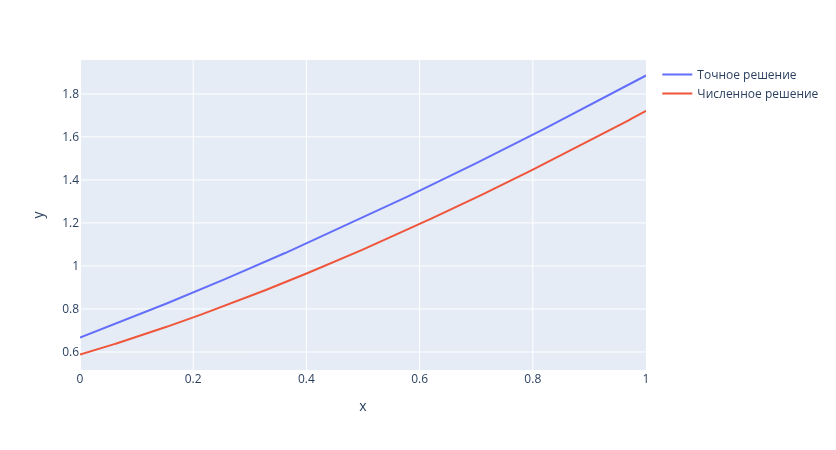
\includegraphics[width=\textwidth]{images/10.png}
            \caption{Сравнение точного и численного решений}
        \end{subfigure}
        \hfill
        \begin{subfigure}[b]{\textwidth}
            \centering
            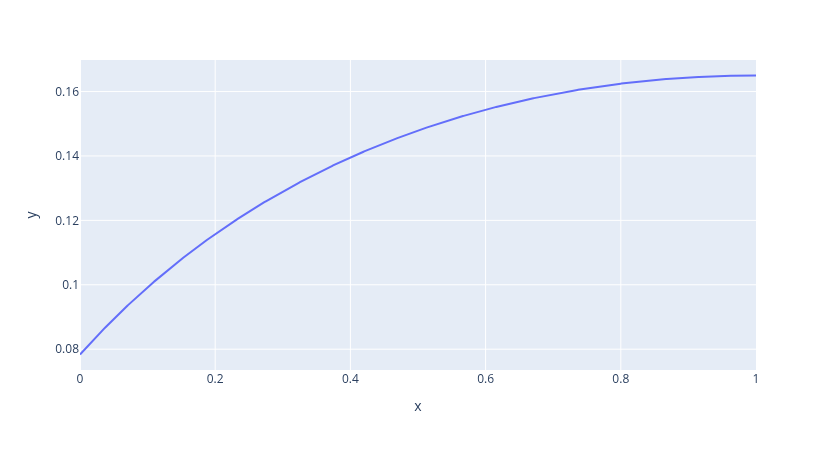
\includegraphics[width=\textwidth]{images/error10.png}
            \caption{Абсолютная погрешность решения}
        \end{subfigure}
        
        \caption{Тестирование решения при $N = 10$}
    \end{figure}

    \begin{figure}[htbp]
        \centering
        \begin{subfigure}[b]{\textwidth}
            \centering
            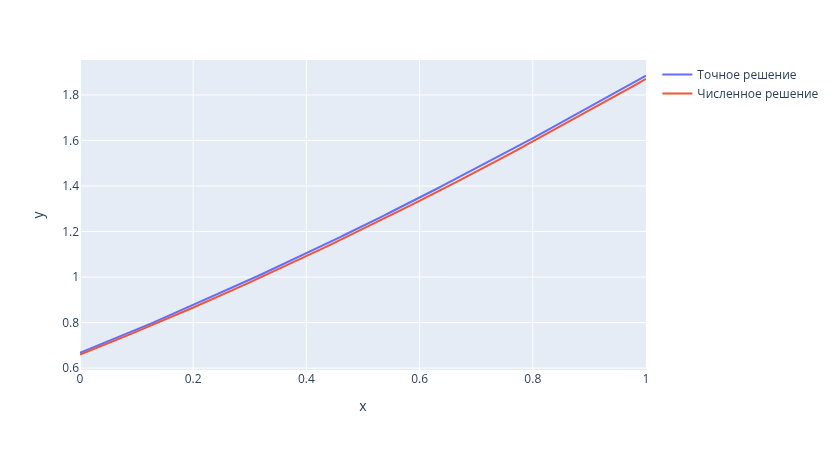
\includegraphics[width=\textwidth]{images/100.png}
            \caption{Сравнение точного и численного решений}
        \end{subfigure}
        \hfill
        \begin{subfigure}[b]{\textwidth}
            \centering
            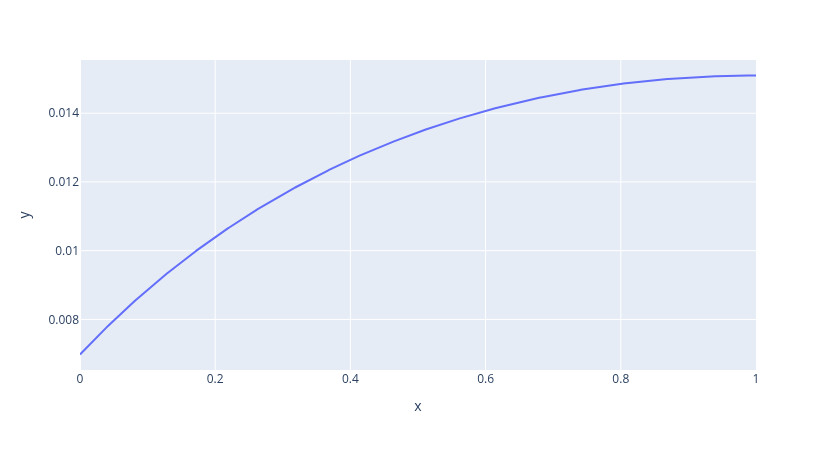
\includegraphics[width=\textwidth]{images/error100.png}
            \caption{Абсолютная погрешность решения}
        \end{subfigure}
        
        \caption{Тестирование решения при $N = 100$}
    \end{figure}

    \begin{figure}[htbp]
        \centering
        \begin{subfigure}[b]{\textwidth}
            \centering
            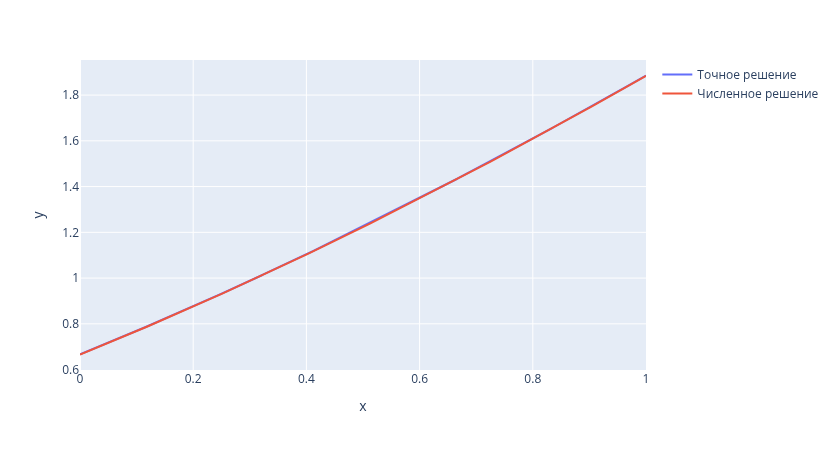
\includegraphics[width=\textwidth]{images/1000.png}
            \caption{Сравнение точного и численного решений}
        \end{subfigure}
        \hfill
        \begin{subfigure}[b]{\textwidth}
            \centering
            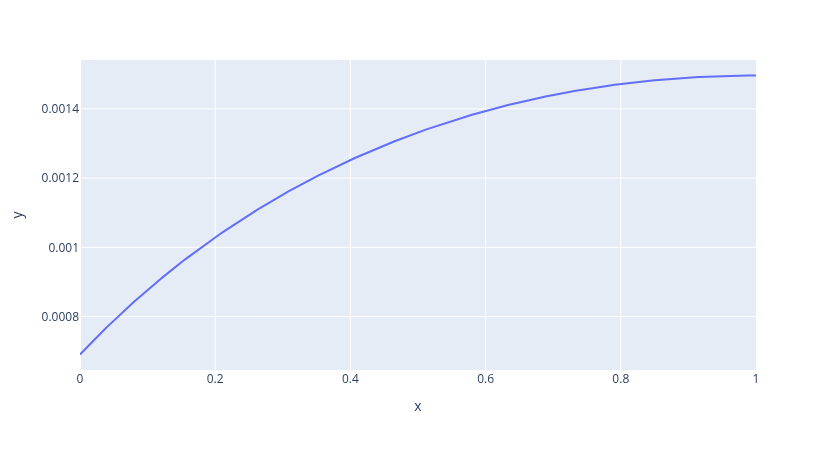
\includegraphics[width=\textwidth]{images/error1000.png}
            \caption{Абсолютная погрешность решения}
        \end{subfigure}
        
        \caption{Тестирование решения при $N = 1000$}
    \end{figure}

    \newpage
    \section{Заключение}

    Метод сплайн-коллокации позволяет не только эффективно аппроксимировать решение, но и одновременно с этим решить задачу интерполяции в отличие от многих других методов, которые дают решение только в узлах.

    \newpage
    \phantomsection
    \addcontentsline{toc}{section}{Список литературы}
    \printbibliography[title={Список литературы}]
\end{document}